\lecture{5}{Graph Neural Networks III: GNN Augmentation and Training}{Tuesday, October 6, 2026}\label{ch:lec05}

% Local TikZ styles (prefix lec05)
\tikzset{
  lec05c/.style={circle, draw=black, thick, fill=white, minimum size=5mm,
                 inner sep=0pt, font=\scriptsize},
  lec05t/.style={circle, draw=black, thick, fill=white, minimum size=3mm,
                 inner sep=0pt},
  lec05num/.style={circle, fill=Red!85!black, draw=white, thick, text=white,
                   minimum size=4.6mm, inner sep=0pt,
                   font=\scriptsize\sffamily\bfseries},
  lec05blk/.style={draw, thick, align=center, font=\small\sffamily,
                   minimum height=9mm, inner sep=3pt},
  lec05lbl/.style={font=\scriptsize\sffamily},
  lec05tr/.style={BrickRed, densely dotted, thick},
  lec05va/.style={Cerulean, densely dotted, thick},
  lec05te/.style={ForestGreen, densely dotted, thick},
  lec05msg/.style={very thick, BrickRed},
  lec05sup/.style={very thick, Orange},
  lec05val/.style={very thick, Cerulean},
  lec05tst/.style={very thick, ForestGreen},
  lec05cut/.style={black!30, densely dotted, thick},
}

\textbf{Outline.} The general GNN framework $\to$ graph manipulation (feature
augmentation, virtual nodes, neighborhood sampling) $\to$ prediction with GNNs
(node-, edge-, graph-level heads) $\to$ training GNNs (labels, loss functions,
evaluation metrics) $\to$ setting up GNN prediction tasks (dataset splits,
transductive vs.\ inductive, link prediction).

% ---------------------------------------------------------------------
\section{Graph manipulation in GNNs}\label{sec:lec05-manip}

\subsection{The general GNN framework; why manipulate graphs}\label{sec:lec05-why}
\slides{9--13}

\begin{itemize}
  \item \textbf{Today: a general GNN framework} (You, Ying, Leskovec,
    \emph{Design Space of Graph Neural Networks}, NeurIPS 2020; figure in
    \cref{ch:lec04}): (1) message, (2) aggregation, (3) layer connectivity,
    (4) graph augmentation, (5) learning objective.
  \item \textbf{(4) Graph manipulation.} Idea: \textbf{raw input graph $\neq$
    computational graph} $\Rightarrow$ graph feature augmentation; graph
    structure manipulation.
  \item \textbf{Our assumption so far:} raw input graph $=$ computational graph.
    \textbf{Reasons for breaking this assumption} and the fixes:
    \cref{tab:lec05-manip}. It's just \textbf{unlikely that the input graph
    happens to be the optimal computation graph} for embeddings.
\end{itemize}

\begin{table}[htbp]
  \centering\small
  \caption{Why and how to manipulate graphs (slides~12--13).}
  \label{tab:lec05-manip}
  \renewcommand{\arraystretch}{1.2}
  \begin{tabularx}{\textwidth}{@{}ll>{\raggedright\arraybackslash}X>{\raggedright\arraybackslash}X@{}}
    \toprule
    Level & The input graph is\dots & Problem & Manipulation\\
    \midrule
    Feature & lacking features & -- & \textbf{feature augmentation} (further
      in Lecture~7)\\
    Structure & too sparse & inefficient message passing & \textbf{add virtual
      nodes / edges}\\
    & too dense & message passing is too costly & \textbf{sample neighbors}
      when doing message passing\\
    & too large & cannot fit the computational graph into a GPU &
      \textbf{sample subgraphs} to compute embeddings (later: scaling up GNNs)\\
    \bottomrule
  \end{tabularx}
\end{table}

\subsection{Feature augmentation}\label{sec:lec05-feat}
\slides{14--19}

\begin{itemize}
  \item \textbf{Why? (1) Input graph does not have node features} -- common
    when we only have the adj.\ matrix. \textbf{Standard approaches:}
    \begin{itemize}
      \item \textbf{a) Assign constant values to nodes} (every node gets
        feature $1$).
      \item \textbf{b) Assign unique IDs to nodes}; these IDs are converted
        into \term{one-hot vectors}. E.g.\ nodes $A,\dots,F$ get IDs $1,\dots,6$
        (total number of IDs $=6$); node with ID $=5$: $[0,0,0,0,1,0]$.
        Comparison: \cref{tab:lec05-onehot}.
    \end{itemize}
\end{itemize}

\begin{table}[htbp]
  \centering\small
  \caption{Feature augmentation: constant vs.\ one-hot (slide~16).}
  \label{tab:lec05-onehot}
  \renewcommand{\arraystretch}{1.2}
  \begin{tabularx}{\textwidth}{@{}>{\raggedright\arraybackslash}p{2.7cm}>{\raggedright\arraybackslash}X>{\raggedright\arraybackslash}X@{}}
    \toprule
    & Constant node feature & One-hot node feature\\
    \midrule
    Expressive power & \textbf{Medium.} All the nodes are identical, but GNN
      can still learn from the graph structure
      & \textbf{High.} Each node has a unique ID, so node-specific information
      can be stored\\
    Inductive learning (generalize to unseen nodes)
      & \textbf{High.} Simple to generalize to new nodes: we assign constant
      feature to them, then apply our GNN
      & \textbf{Low.} Cannot generalize to new nodes: new nodes introduce new
      IDs, GNN doesn't know how to embed unseen IDs\\
    Computational cost & \textbf{Low.} Only 1 dimensional feature
      & \textbf{High.} High dimensional feature, cannot apply to large graphs\\
    Use cases & Any graph, inductive settings (generalize to new nodes)
      & Small graph, transductive settings (no new nodes)\\
    \bottomrule
  \end{tabularx}
\end{table}

\begin{itemize}
  \item \textbf{Why? (2) Certain structures are hard to learn by GNN.}
    Example: \term{cycle count feature} -- can a GNN learn the length of a
    cycle that $v_1$ resides in? \textbf{Unfortunately, no}
    (\cref{fig:lec05-cycle}):
    \begin{itemize}
      \item $v_1$ \textbf{cannot differentiate which graph it resides in}
        (cycle with length 3, 4, or infinite length), because all the nodes in
        the graph have degree of 2 $\Rightarrow$ the computational graphs will
        be \textbf{the same binary tree}.
    \end{itemize}
  \item \textbf{Solution:} use \textbf{cycle count as augmented node features}
    (You et al., \emph{Identity-aware Graph Neural Networks}, AAAI 2021). We
    start from cycle with length 0: $v_1$ in a cycle with length 3 $\to$
    $[0,0,0,1,0,0]$; length 4 $\to$ $[0,0,0,0,1,0]$.
\end{itemize}

\begin{figure}[htbp]
  \centering
  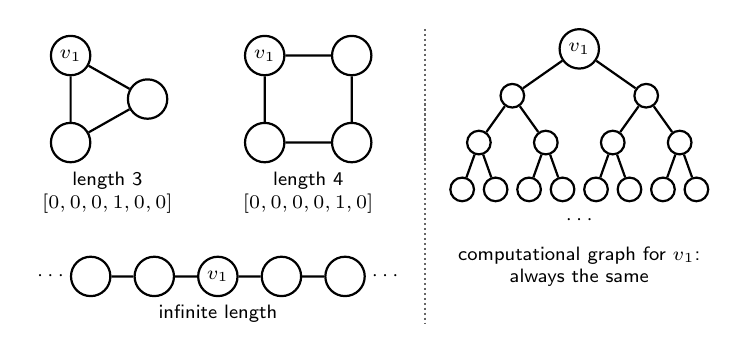
\begin{tikzpicture}[scale=0.85]
    % cycle of length 3
    \node[lec05c] (a1) at (0,1.3) {$v_1$};
    \node[lec05c] (a2) at (0,0) {};
    \node[lec05c] (a3) at (1.15,0.65) {};
    \draw[thick] (a1)--(a2)--(a3)--(a1);
    \node[lec05lbl, align=center] at (0.55,-0.75)
      {length 3\\$[0,0,0,1,0,0]$};
    % cycle of length 4
    \node[lec05c] (b1) at (2.9,1.3) {$v_1$};
    \node[lec05c] (b2) at (4.2,1.3) {};
    \node[lec05c] (b3) at (4.2,0) {};
    \node[lec05c] (b4) at (2.9,0) {};
    \draw[thick] (b1)--(b2)--(b3)--(b4)--(b1);
    \node[lec05lbl, align=center] at (3.55,-0.75)
      {length 4\\$[0,0,0,0,1,0]$};
    % infinite cycle
    \node[lec05c] (c1) at (0.3,-2.0) {};
    \node[lec05c] (c2) at (1.25,-2.0) {};
    \node[lec05c] (c3) at (2.2,-2.0) {$v_1$};
    \node[lec05c] (c4) at (3.15,-2.0) {};
    \node[lec05c] (c5) at (4.1,-2.0) {};
    \draw[thick] (c1)--(c2)--(c3)--(c4)--(c5);
    \node[font=\scriptsize] at (-0.3,-2.0) {$\cdots$};
    \node[font=\scriptsize] at (4.7,-2.0) {$\cdots$};
    \node[lec05lbl] at (2.2,-2.55) {infinite length};
    % separator
    \draw[densely dotted, thick, black!60] (5.3,1.7) -- (5.3,-2.7);
    % computational graph: binary tree
    \node[lec05c] (r) at (7.6,1.4) {$v_1$};
    \foreach \i/\x in {1/6.6, 2/8.6}
      {\node[lec05t] (p\i) at (\x,0.7) {}; \draw[thick] (r)--(p\i);}
    \foreach \i/\x/\p in {1/6.1/1, 2/7.1/1, 3/8.1/2, 4/9.1/2}
      {\node[lec05t] (q\i) at (\x,0.0) {}; \draw[thick] (p\p)--(q\i);}
    \foreach \x/\p in {5.85/1, 6.35/1, 6.85/2, 7.35/2, 7.85/3, 8.35/3,
                       8.85/4, 9.35/4}
      {\node[lec05t] (z) at (\x,-0.7) {}; \draw[thick] (q\p)--(z);}
    \node[font=\scriptsize] at (7.6,-1.15) {$\cdots$};
    \node[lec05lbl, align=center] at (7.6,-1.85)
      {computational graph for $v_1$:\\always the same};
  \end{tikzpicture}
  \caption{$v_1$ in cycles with length 3, 4 and infinite length: all nodes have
  degree 2, so $v_1$ always gets the same computational graph (binary tree);
  the cycle-count features below the cycles separate them (slides~17--19).}
  \label{fig:lec05-cycle}
\end{figure}

\subsection{Structure augmentation: virtual nodes}\label{sec:lec05-virtual}
\slides{20}

\begin{itemize}
  \item \textbf{Motivation:} augment sparse graphs. \textbf{(2) Add virtual
    nodes:} the \term{virtual node} will connect to all the nodes in the graph.
    \begin{itemize}
      \item Suppose in a sparse graph two nodes have shortest path distance of
        10; after adding the virtual node, \textbf{all the nodes will have a
        distance of 2} (node A -- virtual node -- node B).
      \item \textbf{Benefits:} greatly \textbf{improves message passing in
        sparse graphs}.
    \end{itemize}
\end{itemize}

\subsection{Node neighborhood sampling}\label{sec:lec05-sampling}
\slides{21--24}

\begin{itemize}
  \item \textbf{Our approach so far:} all the neighbors are used for message
    passing. \textbf{Problem:} dense/large graphs, high-degree nodes.
  \item \textbf{New idea:} (randomly) determine a node's neighborhood for
    message passing (Hamilton et al., \emph{Inductive Representation Learning
    on Large Graphs}, NeurIPS 2017).
  \item \textbf{Example} (target node $A$ with neighbors $B,C,D$): randomly
    choose 2 neighbors to pass messages $\Rightarrow$ only $B$ and $D$ pass a
    message to $A$. Next time we compute the embeddings, we can sample
    different neighbors $\Rightarrow$ only $C$ and $D$ (slide~24: $B,C$ kept,
    $D$ dropped).
  \item \textbf{In expectation}, we get embeddings similar to the case where
    all the neighbors are used (Ying et al., \emph{Graph Convolutional Neural
    Networks for Web-Scale Recommender Systems}, KDD 2018).
    \textbf{Benefits:} greatly reduce computational cost. And in practice it
    works great!
\end{itemize}

% ---------------------------------------------------------------------
\section{Prediction with GNNs}\label{sec:lec05-pred}

\subsection{The GNN training pipeline}\label{sec:lec05-pipeline}
\slides{26--29}

\begin{itemize}
  \item \textbf{(5) Learning objective.} Next: how do we train a GNN?
  \item \textbf{GNN training pipeline} (\cref{fig:lec05-pipeline}): input graph
    $\to$ GNN $\to$ node embeddings (so far what we have covered) $\to$
    prediction head $\to$ predictions; predictions + labels $\to$ loss function
    and evaluation metrics.
  \item \textbf{Output of a GNN:} set of node embeddings
    $\{\vh_v^{(L)},\forall v\in G\}$.
  \item \textbf{(1) Different prediction heads:} node-level, edge-level and
    graph-level tasks. \textbf{Idea:} different task levels require different
    prediction heads (prediction from one node / from a pair of nodes / from
    the whole graph).
\end{itemize}

\begin{figure}[htbp]
  \centering
  \begin{tikzpicture}[scale=0.85]
    \node[lec05blk] (in) at (0,0) {Input\\graph};
    \node[lec05blk] (gnn) at (2.35,0) {Graph neural\\network};
    \node[lec05blk] (emb) at (4.9,0) {Node\\embeddings};
    \node[lec05blk, text=BrickRed] (head) at (7.75,0) {Prediction\\head};
    \node[lec05blk] (pred) at (10.2,0) {Predictions};
    \node[lec05blk, text=BrickRed] (lab) at (12.45,0) {Labels};
    \node[lec05blk, text=BrickRed] (met) at (11.35,1.75) {Evaluation\\metrics};
    \node[lec05blk, text=BrickRed] (loss) at (11.35,-1.75) {Loss\\function};
    \foreach \a/\b in {in/gnn, gnn/emb, emb/head, head/pred}
      \draw[arrow] (\a) -- (\b);
    \draw[arrow] (pred.north) -- (met.south west);
    \draw[arrow] (lab.north) -- (met.south east);
    \draw[arrow] (pred.south) -- (loss.north west);
    \draw[arrow] (lab.south) -- (loss.north east);
    \node[draw=BrickRed, densely dotted, thick, inner sep=5pt,
          fit=(in)(gnn)(emb)] (sofar) {};
    \node[lec05lbl, anchor=north] at (sofar.south)
      {so far covered; output $\{\vh_v^{(L)},\forall v\in G\}$};
    \node[lec05lbl, anchor=south, text=BrickRed] at (sofar.north)
      {(5) dataset split: train / validation / test};
    \node[lec05lbl, anchor=north, align=center, text=BrickRed] at (head.south)
      {(1) node / edge /\\graph level};
    \node[lec05lbl, anchor=west, align=left, text=BrickRed]
      at ([xshift=3pt]lab.east) {(2) supervised /\\unsupervised};
    \node[lec05lbl, anchor=west, align=left, text=BrickRed]
      at ([xshift=3pt]loss.east) {(3) classification /\\regression loss};
    \node[lec05lbl, anchor=west, align=left, text=BrickRed]
      at ([xshift=3pt]met.east) {(4) accuracy,\\ROC AUC, \dots};
  \end{tikzpicture}
  \caption{GNN training pipeline; (1)--(5) are the parts covered in this
  lecture (slides~27--28, 39, 43, 48, 55, 73).}
  \label{fig:lec05-pipeline}
\end{figure}

\subsection{Prediction heads: node-level}\label{sec:lec05-nodehead}
\slides{30}

\begin{itemize}
  \item \textbf{Node-level prediction:} we can directly make prediction using
    node embeddings! After GNN computation, we have $d$-dim node embeddings
    $\{\vh_v^{(L)}\in\R^d,\forall v\in G\}$.
  \item Suppose we want to make \textbf{$k$-way prediction}: classification
    (classify among $k$ categories) or regression (regress on $k$ targets):
\end{itemize}
\begin{equation}\label{eq:lec05-headnode}
  \hat{\vy}_v = \mathrm{Head}_{\mathrm{node}}\big(\vh_v^{(L)}\big)
  = \mW^{(H)}\vh_v^{(L)}
\end{equation}
\begin{itemize}
  \item[] $\mW^{(H)}\in\R^{k\times d}$: we map node embeddings from
    $\vh_v^{(L)}\in\R^d$ to $\hat{\vy}_v\in\R^k$ so that we can compute the
    loss.
\end{itemize}

\subsection{Prediction heads: edge-level}\label{sec:lec05-edgehead}
\slides{31--33}

\begin{itemize}
  \item \textbf{Edge-level prediction:} make prediction using pairs of node
    embeddings; $k$-way prediction (slide figure: $\vh_u^{(L)}$ at $D$,
    $\vh_v^{(L)}$ at $E$, edge $D$--$E$ = ?):
\end{itemize}
\begin{equation}\label{eq:lec05-headedge}
  \hat{\vy}_{uv} = \mathrm{Head}_{\mathrm{edge}}\big(\vh_u^{(L)},\vh_v^{(L)}\big)
\end{equation}
\begin{itemize}
  \item \textbf{Options for $\mathrm{Head}_{\mathrm{edge}}$. (1) Concatenation
    + Linear} -- we have seen this in graph attention (\cref{ch:lec04});
    \cref{fig:lec05-edgehead}:
\end{itemize}
\begin{equation}\label{eq:lec05-concat}
  \hat{\vy}_{uv} = \mathrm{Linear}\big(\mathrm{Concat}(\vh_u^{(L)},\vh_v^{(L)})\big)
\end{equation}
\begin{itemize}
  \item[] Here $\mathrm{Linear}(\cdot)$ maps $2d$-dimensional embeddings (since
    we concatenated embeddings) to $k$-dim embeddings ($k$-way prediction).
  \item \textbf{(2) Dot product:}
\end{itemize}
\begin{equation}\label{eq:lec05-dot}
  \hat{\vy}_{uv} = \big(\vh_u^{(L)}\big)\tp\vh_v^{(L)}
\end{equation}
\begin{itemize}
  \item[] \textbf{This approach only applies to 1-way prediction} (e.g.\ link
    prediction: predict the existence of an edge).
  \item \textbf{Applying to $k$-way prediction:} similar to \textbf{multi-head
    attention} ($\mW^{(1)},\dots,\mW^{(k)}$ trainable):
\end{itemize}
\begin{align}
  \hat{\vy}_{uv}^{(1)} &= \big(\vh_u^{(L)}\big)\tp\mW^{(1)}\vh_v^{(L)},\ \
    \dots,\ \ \hat{\vy}_{uv}^{(k)} = \big(\vh_u^{(L)}\big)\tp\mW^{(k)}\vh_v^{(L)}
    \label{eq:lec05-dotk}\\
  \hat{\vy}_{uv} &= \mathrm{Concat}\big(\hat{\vy}_{uv}^{(1)},\dots,
    \hat{\vy}_{uv}^{(k)}\big)\in\R^k \notag
\end{align}

\begin{figure}[htbp]
  \centering
  \begin{tikzpicture}[scale=0.85]
    \draw[thick, fill=BrickRed!80] (0,0) rectangle (0.28,0.9);
    \draw[thick, fill=Goldenrod!80] (1.0,0) rectangle (1.28,0.9);
    \node[below, font=\scriptsize] at (0.14,0) {$\vh_u^{(L)}$};
    \node[below, font=\scriptsize] at (1.14,0) {$\vh_v^{(L)}$};
    \draw[densely dotted, thick, -{Stealth[length=2mm]}] (1.55,0.45) --
      node[above, lec05lbl, font=\scriptsize\sffamily\bfseries] {Concatenate}
      (3.35,0.45);
    \draw[thick, fill=BrickRed!80] (3.6,0.45) rectangle (3.88,1.35);
    \draw[thick, fill=Goldenrod!80] (3.6,-0.45) rectangle (3.88,0.45);
    \node[below, font=\scriptsize] at (3.74,-0.45) {$2d$};
    \draw[densely dotted, thick, -{Stealth[length=2mm]}] (4.2,0.45) --
      node[above, font=\scriptsize\sffamily\bfseries] {Linear} (5.7,0.45);
    \node[right] at (5.75,0.45) {$\hat{\vy}_{uv}\in\R^k$};
  \end{tikzpicture}
  \caption{Edge-level head (1): concatenation + linear (slide~32).}
  \label{fig:lec05-edgehead}
\end{figure}

\subsection{Prediction heads: graph-level}\label{sec:lec05-graphhead}
\slides{34--37}

\begin{itemize}
  \item \textbf{Graph-level prediction:} make prediction using all the node
    embeddings in our graph; $k$-way prediction:
\end{itemize}
\begin{equation}\label{eq:lec05-headgraph}
  \hat{\vy}_G = \mathrm{Head}_{\mathrm{graph}}\big(\{\vh_v^{(L)}\in\R^d,
  \forall v\in G\}\big)
\end{equation}
\begin{itemize}
  \item $\mathrm{Head}_{\mathrm{graph}}(\cdot)$ \textbf{is similar to
    $\AGG(\cdot)$ in a GNN layer!}
  \item \textbf{Options} (Xu*, Hu*, Leskovec, Jegelka, \emph{How Powerful Are
    Graph Neural Networks}, ICLR 2019):
\end{itemize}
\begin{align}
  \text{(1) \textbf{Global mean pooling}:}\quad
    & \hat{\vy}_G = \mathrm{Mean}\big(\{\vh_v^{(L)}\in\R^d,\forall v\in G\}\big)
    \label{eq:lec05-mean}\\
  \text{(2) \textbf{Global max pooling}:}\quad
    & \hat{\vy}_G = \mathrm{Max}\big(\{\vh_v^{(L)}\in\R^d,\forall v\in G\}\big)
    \label{eq:lec05-max}\\
  \text{(3) \textbf{Global sum pooling}:}\quad
    & \hat{\vy}_G = \mathrm{Sum}\big(\{\vh_v^{(L)}\in\R^d,\forall v\in G\}\big)
    \label{eq:lec05-sum}
\end{align}
\begin{itemize}
  \item These options work great for \textbf{small graphs}. \textbf{Can we do
    better for large graphs?}
  \item \textbf{Issue of global pooling:} global pooling over a (large) graph
    will lose information.
\end{itemize}
\begin{example}[Toy example: 1-dim node embeddings]
  Node embeddings for $G_1$: $\{-1,-2,0,1,2\}$; for $G_2$:
  $\{-10,-20,0,10,20\}$. Clearly very different node embeddings $\to$ their
  structures should be different. If we do global sum pooling:
  \[
    G_1:\ \hat{y}_G = \mathrm{Sum}(\{-1,-2,0,1,2\}) = 0,\qquad
    G_2:\ \hat{y}_G = \mathrm{Sum}(\{-10,-20,0,10,20\}) = 0
  \]
  $\Rightarrow$ we cannot differentiate $G_1$ and $G_2$!
\end{example}
\begin{itemize}
  \item \textbf{Add virtual super node:} to embed a graph, add a
    \term{virtual super node} that connects to all the nodes in the graph.
    \textbf{Benefits:} GNN learns how to encode the entire input graph.
\end{itemize}

% ---------------------------------------------------------------------
\section{Training graph neural networks}\label{sec:lec05-train}

\subsection{Predictions and labels}\label{sec:lec05-labels}
\slides{39--42}

\begin{itemize}
  \item \textbf{(2) Where does ground-truth come from?} Supervised labels;
    unsupervised signals.
  \item \term{Supervised learning on graphs}: \textbf{labels come from external
    sources}, e.g.\ predict drug likeness of a molecular graph.
  \item \term{Unsupervised learning on graphs}: \textbf{signals come from graphs
    themselves}, e.g.\ link prediction: predict if two nodes are connected.
  \item \textbf{Sometimes the differences are blurry:} we still have
    ``supervision'' in unsupervised learning, e.g.\ train a GNN to predict node
    clustering coefficient. An alternative name for ``unsupervised'' is
    \term{self-supervised}.
  \item \textbf{Supervised labels come from the specific use cases}
    (\cref{tab:lec05-labels}). \textbf{Advice:} reduce your task to node / edge
    / graph labels, since they are easy to work with; e.g.\ we knew some nodes
    form a cluster $\Rightarrow$ treat the cluster that a node belongs to as a
    \textbf{node label}.
  \item \textbf{Unsupervised signals.} Problem: sometimes \textbf{we only have
    a graph, without any external labels}. Solution: ``self-supervised
    learning'' -- we can find supervision signals within the graph, i.e.\ let
    the GNN predict graph quantities (\cref{tab:lec05-labels}). \textbf{These
    tasks do not require any external labels!}
\end{itemize}

\begin{table}[htbp]
  \centering\small
  \caption{Supervised labels vs.\ self-supervised signals at each level
  (slides~41--42).}
  \label{tab:lec05-labels}
  \renewcommand{\arraystretch}{1.2}
  \begin{tabularx}{\textwidth}{@{}l>{\raggedright\arraybackslash}X>{\raggedright\arraybackslash}X@{}}
    \toprule
    Level & Supervised label (from the use case) & Self-supervised signal (let
      the GNN predict)\\
    \midrule
    Node $y_v$ & citation network: which subject area does a node belong to
      & node statistics: such as clustering coefficient, PageRank, \dots\\
    Edge $y_{uv}$ & transaction network: whether an edge is fraudulent
      & link prediction: hide the edge between two nodes, predict if there
      should be a link\\
    Graph $y_G$ & among molecular graphs: the drug likeness of graphs
      & graph statistics: e.g.\ predict if two graphs are isomorphic\\
    \bottomrule
  \end{tabularx}
\end{table}

\subsection{Loss functions}\label{sec:lec05-loss}
\slides{43--47}

\begin{itemize}
  \item \textbf{(3) How do we compute the final loss?} Classification loss;
    regression loss.
  \item \textbf{Setting:} we have $N$ data points; each data point can be a
    node/edge/graph. Node-level: prediction $\hat{\vy}_v^{(i)}$, label
    $\vy_v^{(i)}$; edge-level: $\hat{\vy}_{uv}^{(i)}$, $\vy_{uv}^{(i)}$;
    graph-level: $\hat{\vy}_G^{(i)}$, $\vy_G^{(i)}$. We use prediction
    $\hat{\vy}^{(i)}$, label $\vy^{(i)}$ to refer to \textbf{predictions at all
    levels}.
  \item \term{Classification}: labels $\vy^{(i)}$ with discrete value, e.g.\ node
    classification (which category does a node belong to).
    \term{Regression}: labels $\vy^{(i)}$ with continuous value, e.g.\ predict
    the drug likeness of a molecular graph.
  \item GNNs can be applied to both settings. \textbf{Differences: loss
    function \& evaluation metrics.}
  \item \textbf{Classification loss:} \term{cross entropy (CE)} is a very common
    loss function in classification. $K$-way prediction for $i$-th data point
    ($j$ = $j$-th class); total loss over all $N$ training examples:
\end{itemize}
\begin{equation}\label{eq:lec05-ce}
  \mathrm{CE}\big(\vy^{(i)},\hat{\vy}^{(i)}\big)
  = -\sum_{j=1}^{K}\vy_j^{(i)}\log\big(\hat{\vy}_j^{(i)}\big),
  \qquad
  \mathrm{Loss} = \sum_{i=1}^{N}\mathrm{CE}\big(\vy^{(i)},\hat{\vy}^{(i)}\big)
\end{equation}
\begin{itemize}
  \item[] $\vy^{(i)}\in\R^K$ = one-hot label encoding (e.g.\ $[0,0,1,0,0]$);
    $\hat{\vy}^{(i)}\in\R^K$ = prediction after $\mathrm{Softmax}(\cdot)$
    (e.g.\ $[0.1,0.3,0.4,0.1,0.1]$).
  \item \textbf{Regression loss:} for regression tasks we often use
    \term{Mean Squared Error (MSE)} a.k.a.\ \term{L2 loss}. $K$-way regression
    for data point $(i)$ ($j$ = $j$-th target); total loss over all $N$
    training examples:
\end{itemize}
\begin{equation}\label{eq:lec05-mse}
  \mathrm{MSE}\big(\vy^{(i)},\hat{\vy}^{(i)}\big)
  = \sum_{j=1}^{K}\big(\vy_j^{(i)}-\hat{\vy}_j^{(i)}\big)^2,
  \qquad
  \mathrm{Loss} = \sum_{i=1}^{N}\mathrm{MSE}\big(\vy^{(i)},\hat{\vy}^{(i)}\big)
\end{equation}
\begin{itemize}
  \item[] $\vy^{(i)}\in\R^k$ = real valued vector of targets (e.g.\
    $[1.4,2.3,1.0,0.5,0.6]$); $\hat{\vy}^{(i)}\in\R^k$ = real valued vector of
    predictions (e.g.\ $[0.9,2.8,2.0,0.3,0.8]$).
\end{itemize}

\subsection{Evaluation metrics}\label{sec:lec05-metrics}
\slides{48--53}

\begin{itemize}
  \item \textbf{(4) How do we measure the success of a GNN?} Accuracy; ROC AUC.
  \item We use \textbf{standard evaluation metrics} for GNN (content can be
    found in any ML course); in practice we use \textbf{sklearn} for
    implementation. Suppose we make predictions for $N$ data points.
  \item \textbf{Regression tasks on graphs:} \term{root mean square error
    (RMSE)} and \term{mean absolute error (MAE)}:
\end{itemize}
\begin{equation}\label{eq:lec05-rmse}
  \mathrm{RMSE} = \sqrt{\sum_{i=1}^{N}\frac{\big(\vy^{(i)}-\hat{\vy}^{(i)}\big)^2}{N}},
  \qquad
  \mathrm{MAE} = \frac{\sum_{i=1}^{N}\big|\vy^{(i)}-\hat{\vy}^{(i)}\big|}{N}
\end{equation}
\begin{itemize}
  \item \textbf{Classification tasks on graphs. (1) Multi-class
    classification:} we simply report the \term{accuracy}:
\end{itemize}
\begin{equation}\label{eq:lec05-acc}
  \frac{1\big[\argmax\big(\hat{\vy}^{(i)}\big)=\vy^{(i)}\big]}{N}
\end{equation}
\begin{caution}
  Slide~50 omits the sum over data points; correct:
  $\frac{1}{N}\sum_{i=1}^{N}1\big[\argmax(\hat{\vy}^{(i)})=\vy^{(i)}\big]$.
\end{caution}
\begin{itemize}
  \item \textbf{(2) Binary classification:}
    \begin{itemize}
      \item Metrics \textbf{sensitive to classification threshold}: accuracy;
        precision / recall. If the range of prediction is $[0,1]$, we use $0.5$
        as threshold.
      \item Metric \textbf{agnostic to classification threshold}: \textbf{ROC
        AUC}.
    \end{itemize}
  \item \textbf{Metrics for binary classification} (confusion matrix in
    \cref{fig:lec05-metrics}; sklearn classification report):
\end{itemize}
\begin{align}
  \text{Accuracy} &= \frac{\mathrm{TP}+\mathrm{TN}}{\mathrm{TP}+\mathrm{TN}
    +\mathrm{FP}+\mathrm{FN}} = \frac{\mathrm{TP}+\mathrm{TN}}{|\text{Dataset}|}
    \label{eq:lec05-binacc}\\
  \text{Precision (P)} &= \frac{\mathrm{TP}}{\mathrm{TP}+\mathrm{FP}},\qquad
  \text{Recall (R)} = \frac{\mathrm{TP}}{\mathrm{TP}+\mathrm{FN}},\qquad
  \text{F1-Score} = \frac{2\mathrm{P}*\mathrm{R}}{\mathrm{P}+\mathrm{R}}
    \label{eq:lec05-prf}
\end{align}
\begin{itemize}
  \item \term{ROC curve}: captures the tradeoff in TPR and FPR \textbf{as the
    classification threshold is varied for a binary classifier}. The dashed
    line represents \textbf{performance of a random classifier} (slide plot:
    three classifiers' curves above the diagonal).
\end{itemize}
\begin{equation}\label{eq:lec05-tpr}
  \mathrm{TPR} = \mathrm{Recall} = \frac{\mathrm{TP}}{\mathrm{TP}+\mathrm{FN}},
  \qquad
  \mathrm{FPR} = \frac{\mathrm{FP}}{\mathrm{FP}+\mathrm{TN}}
\end{equation}
\begin{itemize}
  \item \term{ROC AUC}: \textbf{area under the ROC curve}. \textbf{Intuition:}
    the probability that a classifier will rank a randomly chosen positive
    instance higher than a randomly chosen negative one.
\end{itemize}

\begin{figure}[htbp]
  \centering
  \begin{minipage}[c]{0.6\textwidth}
    \centering\small
    \renewcommand{\arraystretch}{1.25}
    \begin{tabular}{@{}>{\raggedright\arraybackslash}p{2.2cm}|>{\centering\arraybackslash}p{2.3cm}|>{\centering\arraybackslash}p{2.3cm}@{}}
      & Actually positive (1) & Actually negative (0)\\
      \hline
      Predicted positive (1) & True positives (TPs) & False positives (FPs)\\
      \hline
      Predicted negative (0) & False negatives (FNs) & True negatives (TNs)\\
    \end{tabular}
  \end{minipage}\hfill
  \begin{minipage}[c]{0.36\textwidth}
    \centering
    \begin{tikzpicture}[scale=0.85]
      \fill[SkyBlue!25] (0,0) .. controls (0.25,1.9) and (0.9,2.5) ..
        (2.6,2.6) -- (2.6,0) -- cycle;
      \draw[-{Stealth[length=2mm]}] (0,0) -- (2.95,0);
      \draw[-{Stealth[length=2mm]}] (0,0) -- (0,2.95);
      \draw[densely dashed, BrickRed!70] (0,0) -- (2.6,2.6);
      \draw[very thick, keyblue] (0,0) .. controls (0.25,1.9) and (0.9,2.5) ..
        (2.6,2.6);
      \node[font=\scriptsize, below] at (0,0) {0};
      \node[font=\scriptsize, below] at (2.6,0) {1};
      \node[font=\scriptsize, left] at (0,2.6) {1};
      \node[lec05lbl, below] at (1.3,-0.05) {FPR};
      \node[lec05lbl, rotate=90, above] at (-0.05,1.3) {TPR};
      \node[lec05lbl] at (2.0,0.55) {AUC};
      \node[lec05lbl, rotate=45, text=BrickRed!80, anchor=north]
        at (1.45,1.4) {random};
    \end{tikzpicture}
  \end{minipage}
  \caption{Confusion matrix (slide~51) and ROC curve: TPR vs.\ FPR as the
  threshold varies, diagonal = random classifier, shaded area = ROC AUC
  (slides~52--53).}
  \label{fig:lec05-metrics}
\end{figure}

% ---------------------------------------------------------------------
\section{Setting up GNN prediction tasks}\label{sec:lec05-setup}

\subsection{Dataset split: fixed vs.\ random}\label{sec:lec05-fixed}
\slides{55--56}

\begin{itemize}
  \item \textbf{(5) How do we split our dataset into train / validation / test
    set?}
  \item \term{Fixed split}: we will split our dataset \textbf{once}.
    \begin{itemize}
      \item \textbf{Training set:} used for optimizing GNN parameters.
      \item \textbf{Validation set:} develop model/hyperparameters.
      \item \textbf{Test set:} held out until we report final performance.
    \end{itemize}
  \item \textbf{A concern:} sometimes we cannot guarantee that the test set
    will really be held out.
  \item \term{Random split}: we will \textbf{randomly split} our dataset into
    training / validation / test; we report \textbf{average performance over
    different random seeds}.
\end{itemize}

\subsection{Why splitting graphs is special}\label{sec:lec05-special}
\slides{57--61}

\begin{itemize}
  \item \textbf{Image dataset} -- image classification: each data point is an
    image; here \textbf{data points are independent} (image 5 will not affect
    our prediction on image 1).
  \item \textbf{Splitting a graph dataset is different!} Node classification:
    each data point is a node; here \textbf{data points are NOT independent}:
    node 5 will affect our prediction on node 1, because it will participate in
    message passing $\to$ affect node 1's embedding. What are our options?
    (\cref{fig:lec05-nodesplit})
  \item \textbf{Solution 1 (\term{transductive setting}):} the input graph can
    be observed in all the dataset splits (training, validation and test set).
    \textbf{We will only split the (node) labels.}
    \begin{itemize}
      \item At training time, we compute embeddings \textbf{using the entire
        graph}, and train using node 1\&2's labels.
      \item At validation time, we compute embeddings using the entire graph,
        and evaluate on node 3\&4's labels.
    \end{itemize}
  \item \textbf{Solution 2 (\term{inductive setting}):} we \textbf{break the
    edges between splits to get multiple graphs}. Now we have 3 graphs that are
    independent: node 5 will not affect our prediction on node 1 any more.
    \begin{itemize}
      \item At training time, we compute embeddings using the graph over node
        1\&2, and train using node 1\&2's labels.
      \item At validation time, we compute embeddings using the graph over node
        3\&4, and evaluate on node 3\&4's labels.
    \end{itemize}
\end{itemize}

\begin{figure}[htbp]
  \centering
  \begin{tikzpicture}[scale=0.85]
    % legend
    \node[lec05lbl, font=\small\sffamily\bfseries, text=BrickRed, anchor=west]
      at (-3.6,1.1) {Training};
    \node[lec05lbl, font=\small\sffamily\bfseries, text=Cerulean, anchor=west]
      at (-3.6,0.5) {Validation};
    \node[lec05lbl, font=\small\sffamily\bfseries, text=ForestGreen, anchor=west]
      at (-3.6,-0.1) {Test};
    \foreach \sx/\ind/\ttl in {0/0/{(a) transductive:\\entire graph observed},
                               5.0/1/{(b) inductive: edges\\between splits broken}} {
      \begin{scope}[shift={(\sx,0)}]
        \node[lec05num] (n1) at (0,1.0) {1};
        \node[lec05num] (n2) at (1.3,1.25) {2};
        \node[lec05num] (n3) at (2.6,0.9) {3};
        \node[lec05num] (n4) at (2.1,-0.2) {4};
        \node[lec05num] (n5) at (0.9,-0.2) {5};
        \node[lec05num] (n6) at (-0.4,0.15) {6};
        \begin{scope}[on background layer]
          \draw[very thick] (n1)--(n2) (n3)--(n4) (n6)--(n5);
          \ifnum\ind=0
            \draw[very thick] (n2)--(n3) (n1)--(n5) (n2)--(n5) (n2)--(n4)
              (n5)--(n4);
          \else
            \draw[lec05cut] (n2)--(n3) (n1)--(n5) (n2)--(n5) (n2)--(n4)
              (n5)--(n4);
          \fi
        \end{scope}
        \draw[lec05tr, rotate around={10.9:(0.65,1.125)}]
          (0.65,1.125) ellipse (1.0 and 0.36);
        \draw[lec05va, rotate around={65.6:(2.35,0.35)}]
          (2.35,0.35) ellipse (0.97 and 0.34);
        \draw[lec05te, rotate around={-15.1:(0.25,-0.025)}]
          (0.25,-0.025) ellipse (1.03 and 0.36);
        \node[lec05lbl, align=center, anchor=north] at (1.1,-0.7) {\ttl};
      \end{scope}
    }
  \end{tikzpicture}
  \caption{Splitting node classification on one graph: training $\{1,2\}$,
  validation $\{3,4\}$, test $\{5,6\}$ (slides~58--60).}
  \label{fig:lec05-nodesplit}
\end{figure}

\begin{table}[htbp]
  \centering\small
  \caption{Transductive vs.\ inductive settings (slide~61).}
  \label{tab:lec05-settings}
  \renewcommand{\arraystretch}{1.2}
  \begin{tabularx}{\textwidth}{@{}>{\raggedright\arraybackslash}p{2.4cm}>{\raggedright\arraybackslash}X>{\raggedright\arraybackslash}X@{}}
    \toprule
    & \textbf{Transductive setting} & \textbf{Inductive setting}\\
    \midrule
    Train / val / test sets & on the \textbf{same graph} & on \textbf{different
      graphs}\\
    Dataset & consists of \textbf{one graph} & consists of \textbf{multiple
      graphs}\\
    What each split sees & the entire graph can be observed in all dataset
      splits; we only split the labels
      & each split can only observe the graph(s) within the split; a successful
      model should \textbf{generalize to unseen graphs}\\
    Tasks & only applicable to \textbf{node / edge} prediction tasks
      & applicable to \textbf{node / edge / graph} tasks\\
    \bottomrule
  \end{tabularx}
\end{table}

\subsection{Examples: node and graph classification}\label{sec:lec05-nodegraph}
\slides{62--63}

\begin{itemize}
  \item \textbf{Transductive node classification:} all the splits can observe
    the entire graph structure, but can only observe the labels of their
    respective nodes (e.g.\ training $\{B,C,F\}$, validation $\{A,D\}$, test
    $\{E\}$ on one graph).
  \item \textbf{Inductive node classification:} suppose we have a dataset of 3
    graphs; each split contains an independent graph.
  \item \textbf{Graph classification:} only the \textbf{inductive setting} is
    well defined, because \textbf{we have to test on unseen graphs}. E.g.\ a
    dataset of 5 graphs: each split will contain independent graph(s) (3
    training, 1 validation, 1 test).
\end{itemize}

\subsection{Example: link prediction; the full pipeline}\label{sec:lec05-link}
\slides{64--73}

\begin{itemize}
  \item \textbf{Goal of link prediction:} predict missing edges.
  \item \textbf{Setting up link prediction is tricky:} link prediction is an
    unsupervised / self-supervised task $\Rightarrow$ we need to \textbf{create
    the labels and dataset splits} on our own. Concretely, \textbf{hide some
    edges from the GNN} and \textbf{let the GNN predict if the edges exist}
    (original graph $\to$ input graph to GNN $\to$ predictions made by GNN).
  \item For link prediction, \textbf{we will split edges twice}. \textbf{Step
    1: assign 2 types of edges in the original graph}
    (\cref{fig:lec05-linksplit}a):
    \begin{itemize}
      \item \term{Message edges}: used for GNN message passing.
      \item \term{Supervision edges}: used for computing objectives.
      \item After step 1: only message edges will remain in the graph;
        supervision edges are used as supervision for edge predictions made by
        the model, will not be fed into GNN.
    \end{itemize}
  \item \textbf{Step 2: split edges into train / validation / test.}
  \item \textbf{Option 1: inductive link prediction split.} Suppose we have a
    dataset of 3 graphs; each inductive split will contain an independent graph
    ($G_1$ training, $G_2$ validation, $G_3$ test set). In train or val or test
    set, each graph will have 2 types of edges: message edges + supervision
    edges (e.g.\ $G_1$: message $(1,5),(5,2),(2,3)$, supervision
    $(2,4),(4,3)$). \textbf{Supervision edges are not the input to GNN.}
  \item \textbf{Option 2: transductive link prediction split} -- this is
    \textbf{the default setting} when people talk about link prediction.
    Suppose we have a dataset of 1 graph.
    \begin{itemize}
      \item By definition of ``transductive'', the entire graph can be observed
        in all dataset splits. But since edges are both part of graph structure
        and the supervision, we need to \textbf{hold out validation / test
        edges}.
      \item To train the training set, we further need to \textbf{hold out
        supervision edges for the training set}.
    \end{itemize}
  \item \textbf{Transductive split, exact settings}
    (\cref{fig:lec05-linksplit}b--d):
    \begin{itemize}
      \item (1) At training time: use \textbf{training message edges} to predict
        \textbf{training supervision edges}.
      \item (2) At validation time: use training message edges \& training
        supervision edges to predict \textbf{validation edges}.
      \item (3) At test time: use training message edges \& training
        supervision edges \& validation edges to predict \textbf{test edges}.
    \end{itemize}
  \item \textbf{Why do we use growing number of edges?} After training,
    supervision edges are known to GNN. Therefore, an ideal model should use
    supervision edges in message passing at validation time. The same applies
    to the test time.
  \item \textbf{Summary:} transductive link prediction split $\Rightarrow$
    split graph with \textbf{4 types of edges}: training message edges,
    training supervision edges, validation edges, test edges. \textbf{Note:}
    link prediction settings are tricky and complex; you may find papers do
    link prediction differently. Luckily, we have full support in \textbf{PyG}
    and \textbf{GraphGym}.
\end{itemize}
\begin{caution}
  Slide~72's legend colours validation edges green and test edges blue, the
  reverse of slides~70--71 (there $(5,4)$ is the validation edge and $(2,3)$
  the test edge).
\end{caution}
\begin{itemize}
  \item \textbf{Full pipeline} (slide~73): GNN training pipeline with dataset
    split (\cref{fig:lec05-pipeline}). \textbf{Implementation resources:}
    \textbf{GraphGym} further implements the full pipeline to facilitate GNN
    design.
\end{itemize}

\begin{figure}[htbp]
  \centering
  \begin{tikzpicture}[scale=0.85]
    \foreach \sx/\pn in {0/a, 4.0/b, 8.0/c, 12.0/d} {
      \begin{scope}[shift={(\sx,0)}]
        \node[lec05num] (\pn1) at (0,1.0) {1};
        \node[lec05num] (\pn2) at (1.1,1.35) {2};
        \node[lec05num] (\pn3) at (2.3,1.05) {3};
        \node[lec05num] (\pn5) at (0.4,0) {5};
        \node[lec05num] (\pn4) at (1.6,0) {4};
      \end{scope}
    }
    \begin{scope}[on background layer]
      % (a) step 1: message vs supervision edges
      \draw[very thick] (a1)--(a5) (a5)--(a2) (a2)--(a3) (a5)--(a4);
      \draw[lec05sup] (a2)--(a4) (a4)--(a3);
      % (b) training time
      \draw[lec05msg] (b1)--(b5) (b5)--(b2) (b2)--(b4);
      \draw[Orange, densely dotted, very thick] (b4)--(b3);
      % (c) validation time
      \draw[lec05msg] (c1)--(c5) (c5)--(c2) (c2)--(c4);
      \draw[lec05sup] (c4)--(c3);
      \draw[Cerulean, densely dotted, very thick] (c5)--(c4);
      % (d) test time
      \draw[lec05msg] (d1)--(d5) (d5)--(d2) (d2)--(d4);
      \draw[lec05sup] (d4)--(d3);
      \draw[lec05val] (d5)--(d4);
      \draw[ForestGreen, densely dotted, very thick] (d2)--(d3);
    \end{scope}
    \node[lec05lbl, align=center, anchor=north] at (1.15,-0.4)
      {(a) step 1: message\\(black) vs.\ supervision\\(orange) edges};
    \node[lec05lbl, align=center, anchor=north] at (5.15,-0.4)
      {(b) training: message\\edges $\to$ training\\supervision edges};
    \node[lec05lbl, align=center, anchor=north] at (9.15,-0.4)
      {(c) validation: + training\\supervision $\to$\\validation edges};
    \node[lec05lbl, align=center, anchor=north] at (13.15,-0.4)
      {(d) test: + validation\\edges $\to$ test edges};
    % legend
    \begin{scope}[shift={(2.0,-2.15)}]
      \foreach \x/\sty/\txt in {0/lec05msg/training message,
          3.5/lec05sup/training supervision, 7.6/lec05val/validation,
          10.2/lec05tst/test}
        {\draw[\sty] (\x,0) -- (\x+0.5,0);
         \node[lec05lbl, anchor=west, text height=1.5ex, text depth=0.3ex]
           at (\x+0.55,0) {\txt};}
    \end{scope}
  \end{tikzpicture}
  \caption{Link prediction: message vs.\ supervision edges (slides~64--65) and
  the transductive split at training / validation / test time; dotted = the
  edges being predicted (slides~70--72).}
  \label{fig:lec05-linksplit}
\end{figure}

% ---------------------------------------------------------------------
\bigskip\phantomsection
\addcontentsline{toc}{section}{Lecture 5 at a glance}
\begin{summarybox}[Lecture 5 at a glance]
  \begin{itemize}
    \item \textbf{Graph manipulation:} input graph $\neq$ computational graph.
      No features $\to$ constant (inductive) or one-hot IDs (transductive);
      cycle counts. Sparse $\to$ virtual nodes; dense $\to$ neighbor sampling;
      large $\to$ subgraph sampling.
    \item \textbf{Heads:} node $\hat{\vy}_v=\mW^{(H)}\vh_v^{(L)}$; edge
      $\mathrm{Linear}(\mathrm{Concat}(\vh_u^{(L)},\vh_v^{(L)}))$ or
      $(\vh_u^{(L)})\tp\vh_v^{(L)}$ ($k$-way: $(\vh_u^{(L)})\tp\mW^{(i)}\vh_v^{(L)}$,
      concatenated); graph: global mean / max / sum pooling (loses information
      on large graphs), virtual super node.
    \item \textbf{Labels:} supervised (external) vs.\ unsupervised =
      self-supervised (from the graph itself). \textbf{Loss:}
      $\mathrm{CE}=-\sum_j\vy_j^{(i)}\log\hat{\vy}_j^{(i)}$,
      $\mathrm{MSE}=\sum_j(\vy_j^{(i)}-\hat{\vy}_j^{(i)})^2$, summed over $N$.
    \item \textbf{Metrics:} RMSE, MAE; accuracy; $\mathrm{P}=\frac{\mathrm{TP}}{\mathrm{TP}+\mathrm{FP}}$,
      $\mathrm{R}=\frac{\mathrm{TP}}{\mathrm{TP}+\mathrm{FN}}$,
      $\mathrm{F1}=\frac{2\mathrm{P}\mathrm{R}}{\mathrm{P}+\mathrm{R}}$; ROC
      AUC = area under the TPR-vs.-FPR curve.
    \item \textbf{Splits:} fixed vs.\ random (average over seeds); transductive
      (one graph, split labels; node/edge tasks) vs.\ inductive (multiple
      graphs; node/edge/graph tasks); graph classification is inductive only.
    \item \textbf{Link prediction:} message vs.\ supervision edges; transductive:
      train message $\to$ train supervision; $+$ train sup.\ $\to$ validation;
      $+$ validation $\to$ test.
  \end{itemize}
\end{summarybox}
